
% Sample latex source for the ``Sample Homework'' handout from AMath 586.
% You also need to download macros.tex, err1.eps, err2.eps, err3.eps.

\documentclass{article}
\usepackage{amsmath}
\usepackage{epsfig,psfrag}

\setlength{\textwidth}{6.5in}
\setlength{\textheight}{8.9in}
\setlength{\voffset}{-1in}
\setlength{\oddsidemargin}{0in}
\setlength{\evensidemargin}{0in}


% a few handy macros

\newcommand\matlab{{\sc matlab}}
\newcommand{\goto}{\rightarrow}
\newcommand{\bigo}{{\mathcal O}}
\newcommand{\half}{\frac{1}{2}}
%\newcommand\implies{\quad\Longrightarrow\quad}
\newcommand\reals{{{\rm l} \kern -.15em {\rm R} }}
\newcommand\complex{{\raisebox{.043ex}{\rule{0.07em}{1.56ex}} \hskip -.35em {\rm C}}}


% macros for matrices/vectors:

% matrix environment for vectors or matrices where elements are centered
\newenvironment{mat}{\left[\begin{array}{ccccccccccccccc}}{\end{array}\right]}
\newcommand\bcm{\begin{mat}}
\newcommand\ecm{\end{mat}}

% matrix environment for vectors or matrices where elements are right justifvied
\newenvironment{rmat}{\left[\begin{array}{rrrrrrrrrrrrr}}{\end{array}\right]}
\newcommand\brm{\begin{rmat}}
\newcommand\erm{\end{rmat}}

% for left brace and a set of choices
\newenvironment{choices}{\left\{ \begin{array}{ll}}{\end{array}\right.}
\newcommand\when{&\text{if~}}
\newcommand\otherwise{&\text{otherwise}}
% sample usage:
%  \delta_{ij} = \begin{choices} 1 \when i=j, \\ 0 \otherwise \end{choices}


% for labeling and referencing equations:
\newcommand{\eql}{\begin{equation}\label}
\newcommand{\eqn}[1]{(\ref{#1})}
% can then do
%  \eql{eqnlabel}
%  ...
%  \end{equation}
% and refer to it as equation \eqn{eqnlabel}.  


% some useful macros for finite difference methods:
\newcommand\unp{U^{n+1}}
\newcommand\unm{U^{n-1}}

% for chemical reactions:
\newcommand{\react}[1]{\stackrel{K_{#1}}{\rightarrow}}
\newcommand{\reactb}[2]{\stackrel{K_{#1}}{~\stackrel{\rightleftharpoons}
   {\scriptstyle K_{#2}}}~}

  % define some macros that are generally useful
                % download macros.tex so this file will be found

% some more macros, useful for this document
\newcommand{\sixth}{\frac{1}{6}}  
\newcommand{\bx}{\bar x}

%-------------------------------------------------------------------
\begin{document}          

\hfill\vbox{\hbox{AMath 586}\hbox{Sample Homework}\hbox{Spring, 2007}}

\vskip .3in

\begin{center}\Large\bf 
Format for homework solutions and a sample write-up
\end{center}
\vskip 15pt

Many of the homework problems in this course will have a large
computational component.  I hope that these problems will achieve several
goals, allowing you to obtain
\vskip 4pt

\begin{enumerate}

\item Hands on experience in using various algorithms by writing your own
programs and/or using software.  This should increase your
understanding of the advantages, limitations, and proper use of various
algorithms.

\item Practice in designing numerical experiments and interpreting the
results, both as a computational scientist using a method to study some
physical problem and as a numerical analyst attempting to understand the
behavior of an algorithm.

\item Practice in writing up your results and analysis in a manner that it
can be understood and appreciated by others.
\end{enumerate}

\vskip 4pt

In particular, it is not enough to simply get your program running and hand
in a bunch of output.  Typically you will be
required to make some creative choices in deciding what to run and do some
analysis of your results in order to understand what is going on, or at
least to check that the method is working as expected.  You should also
write up your analysis and conclusions clearly and concisely.

I suggest that you consider using  a format along the following lines, as
modified to fit the particular problem.

\vskip 5pt
\begin{enumerate} 
\item A brief description of the problem.

\vskip 4pt
\item A description of the method you have used to solve it, with
documentation of what choices you have made for any parameters, stepsizes,
error tolerances, etc.

\vskip 4pt
\item Results obtained, presented in a suitable format.  If the solution is
a function then a graph is typically easier to interpret than a long list
of numbers.  If the exact solution is available then a comparison of the
two on the same graph is useful.  Comparision of results with different
parameter choices (e.g., with different step sizes to show convergence) can
often be done on a single graph with good labeling so that it can be
clearly read.  If the error is so small that it is hard to distinguish one
graph from another, a separate graph of the errors (suitably scaled) may be
best.  

\vskip 4pt
Tables of errors are appropriate for checking the convergence rate, but
tables with more than a dozen numbers or so become unwieldy.  In
particular, if the error is a function, then you should print out some
appropriate norm of the error, not the error at every point.  A graph of
the error vs. some parameter (step size, iteration number)
may also be useful. Often a log-log plot is best
for this.

\vskip 4pt
Part of the problem is to choose what output to present.  If you have to
run 100 cases in order to understand what is going on, please don't give me
the output of all 100!  Once you understand things clearly, you should be
able to select a small set of cases that illustrate the main points,
different types of behavior, critical cases, or whatever.  Present results
that illustrate and complement your analysis and conclusions.

\vskip 4pt
\item Analysis of results, e.g., computation of convergence rates from the
computed results.  Also compare your results with the theory, explain any
strange behavior observed, make comparisons of different methods if
relevant, etc.

\vskip 4pt
\item Computer code.  Please attach your code, or at least a sample of it.
If you have several different versions with minor modifications, then one
representative version would be enough.  Please provide some documentation
in the program so that it is possible to figure it out.
\end{enumerate} 

\vskip 10pt
{\bf Typesetting.}
Although not required, I suggest that you use latex to type up your
solutions.  This is the standard math typesetting system used by most
researchers and journals in applied mathematics so it's good to get
proficient at using it.  I will try to make it easy for you to learn it as
we go along if you're not already familiar with it, by providing some
examples of how the sorts of expressions we use in this course are typeset.

The latex source for all the homework assignments will be available
from the webpage so you don't have to retype the exercises, just copy these
into your latex file if you want to include the questions along with your
solutions.

To get started, there are many latex tutorials on the web and many books.  
You might also
want to take a look at the latex source for this handout, available from the
class webpage.

Note: the figures were made using matlab to first display the figure on the
screen and the
\begin{verbatim}
     >> print err1.eps
\end{verbatim}
for example, dumps the current screen to an encapsulated postscript file
that is read into the latex document using {\tt epsfig}.


\vskip 10pt
{\bf Example.} As an example of a reasonable write-up, here is a sample problem and
solution.  The matlab m-files can be obtained from the class web page.

\vskip 10pt
\hrule
\vskip 10pt

\centerline{\Large\bf Problem}
\vskip 10pt

Compute approximations to $u'(\bar x)$ for $\bar x=1$ using the
approximations 
\begin{equation*}
\begin{split} 
D_+u(\bar x) &= \frac{1}{h}[u(\bar x+h)-u(\bar x)]\\
D_0u(\bar x) &= \frac{1}{2h}[u(\bar x+h)-u(\bar x -h)]\\
D_3u(\bar x) &= \frac{1}{6h}[ 2u(\bx+h)+3u(\bx)-6u(\bx-h)+u(\bx-2h)]
\end{split}
\end{equation*} 
for each of the following functions:
\begin{equation*}
\begin{split}
u_1(x) &= \sin(10 x),\\
u_2(x) &= 4x^3-12x^2+14x-4,\\
u_3(x) &= |x-1.001|^{3/2}.
\end{split}
\end{equation*}
In each case use several different values of $h$ to approximate the
derivative
and discuss the behavior of the errors as $h$ is decreased.


\vskip 10pt
\hrule
\vskip 10pt


\centerline{\Large\bf Solution}
\vskip 10pt
Taylor series expansion of the three methods shows that:
\begin{equation*}
\begin{split}
D_+u(\bx) -u'(\bx) &=   \half hu''(\bx) + \sixth h^2
u'''(\bx) + \bigo(h^3)\\
D_0 u(\bx)-u'(\bx) &= \sixth h^2 u'''(\bx)+\bigo(h^4)\\
D_3u(\bx) - u'(\bx) &= \frac{1}{12} h^3 u''''(\bx) + \bigo(h^4).
\end{split}
\end{equation*}
We expect the methods to be first-order, second-order, and third-order
accurate respectively.

\newpage

{\bf First test function:}
For the function $u_1(x)$ we have $u_1'(1) = 10\cos(10) \approx -8.3907$.
Applying each difference approximation
to $u_1(x)$ gives the errors shown in the Table below and
plotted in Figure 1.
Here the values $h=10^{-j}$ for $j=1,~2,~\ldots,~7$ are used.
For larger values of $h$ the errors behave exactly as expected.
Note that reducing $h$ by a factor of 10 reduces the error
in $D_+$ by a factor of roughly 10, in $D_0$ by roughly 100, and in $D_3$ by
roughly 1000.

\begin{verbatim}

             h         D+ error     D_0 error   D_3 error

         1.0000e-01   3.8310e+00   1.3302e+00  -1.3495e-01
         1.0000e-02   2.8576e-01   1.3978e-02  -4.2466e-04
         1.0000e-03   2.7341e-02   1.3984e-04  -4.5055e-07
         1.0000e-04   2.7215e-03   1.3985e-06  -4.4782e-10
         1.0000e-05   2.7202e-04   1.4007e-08   2.4212e-11
         1.0000e-06   2.7201e-05   4.1279e-10   2.4625e-10
         1.0000e-07   2.7116e-06  -6.9743e-10   4.2986e-09


\end{verbatim}


\begin{figure}[h]
\hfil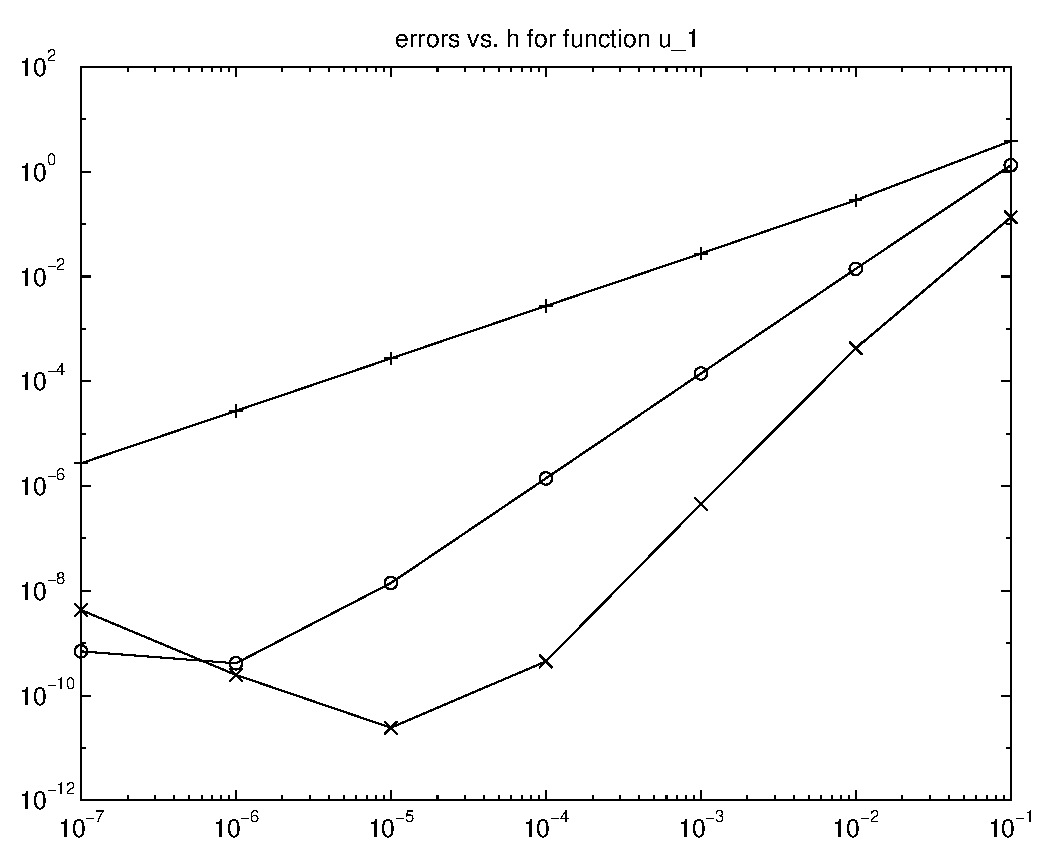
\epsfig{file=err1.eps,width=3in}\hfil
\caption{Log-log plot of errors vs.\ $h$ for first test function $u_1$.
$+=D_+$, $o=D_0$, $\times = D_3$.}
\end{figure}


For smaller values of $h$ the error does not continue to  decrease
in the expected manner.  This is due to the phenomenon of {\it
cancellation}.  Consider $D_0$ for example, with $h=10^{-7}$.  Then we
expect the error to be roughly 
\[
\frac{1}{6} \cdot 10^{-14} \cdot 1000\cos(10) = -1.4 \times 10^{-12}.
\]
However, since $u(\bx+h)$ and $u(\bx-h)$ agree to roughly 6 places, in the
subtraction we lose 6 significant figures.  Since these results were
computed in matlab which uses double precision with about 15 significant
figures, this introduces an error in about the 9'th figure which means we
cannot expect an error that is smaller than about $10^{-9}$, as observed.
The asymptotic error analysis is no longer valid when the rounding errors
dominate.

\vskip 5pt
{\bf NOTE:}  In solving differential equations, rounding errors are rarely
a problem since we do not typically use such small values of $h$.

\newpage
{\bf Second test function:}
With this function we obtain the results shown in Figure 2.
For very small $h$ the results are again contaminated by roundoff.  For
larger $h$ we see some unexpected behavior.  The approximations $D_+$ and
$D_0$ produce essentially the same results while $D_3$ looks to be nearly
exact.  Looking carefully at the truncation errors shows that this is
correct, however.  The function $u_2$ satisfies $u_2''(1)=0$ so that the
leading term in the error for $D_+$ drops out.  Also, since $u_2$ is a
polynomial of degree 3, its 4'th derivative and all higher derivatives are
zero everywhere, so the error in $D_3$ should be zero.  The fact that it
isn't exactly zero is again a result of the rounding errors that arise in
computing $D_3 u_2(1)$.

\begin{verbatim}

             h         D+ error     D_0 error   D_3 error

         1.0000e-01   4.0000e-02   4.0000e-02   7.5495e-15
         1.0000e-02   4.0000e-04   4.0000e-04  -1.2879e-14
         1.0000e-03   4.0000e-06   4.0000e-06   9.6412e-13
         1.0000e-04   3.9999e-08   4.0008e-08   1.3102e-11
         1.0000e-05   4.5719e-10   5.0160e-10   1.4633e-10
         1.0000e-06  -1.4968e-09  -6.0862e-10  -1.6504e-11
         1.0000e-07   5.6086e-09  -3.2732e-09  -1.2155e-08


\end{verbatim}


\begin{figure}[h]
\hfil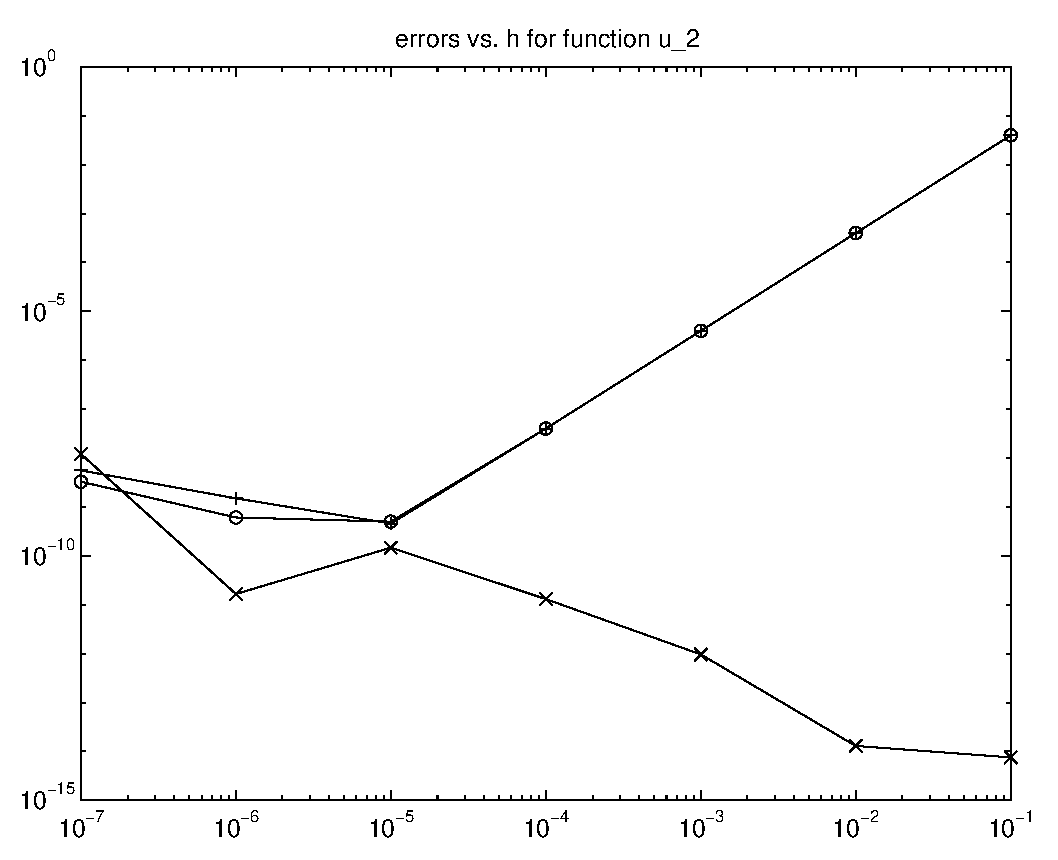
\epsfig{file=err2.eps,width=3in}\hfil
\caption{Log-log plot of errors vs.\ $h$ for test function $u_2$.
$+=D_+$, $o=D_0$, $\times = D_3$.}
\end{figure}


\newpage
{\bf Third test function:}
This function shows the expected asymptotic behavior for sufficiently small
values of $h$ (until cancellation contaminates $D_3$, at least), but does
not show the expected rates for larger values of $h$.  The reason is
because the function $u_3(x)$ is not smooth at the point $x=1.001$.  
The first derivative looks like a square root while the second 
and higher derivatives blow up at this point.
If we difference across a point of nonsmoothness, we cannot expect the
convergence rates based on Taylor series expansions to be valid.  For
$h<10^{-3}$, however, all of the points in the difference formulas are on
the same side of the singularity, the solution is now smooth and we see
the expected rates.

\begin{verbatim}

             h         D+ error     D_0 error   D_3 error

         1.0000e-01   3.5861e-01   4.2691e-02  -1.9368e-02
         1.0000e-02   1.2965e-01   3.2440e-02   1.2827e-02
         1.0000e-03   1.5811e-02   2.7128e-03   1.1890e-03
         1.0000e-04   1.2064e-03   1.9801e-05   1.3533e-06
         1.0000e-05   1.1878e-04   1.9765e-07   1.4678e-09
         1.0000e-06   1.1861e-05   1.9777e-09   9.9724e-13
         1.0000e-07   1.1858e-06   1.8403e-11   1.6190e-11


\end{verbatim}

\begin{figure}[h]
\hfil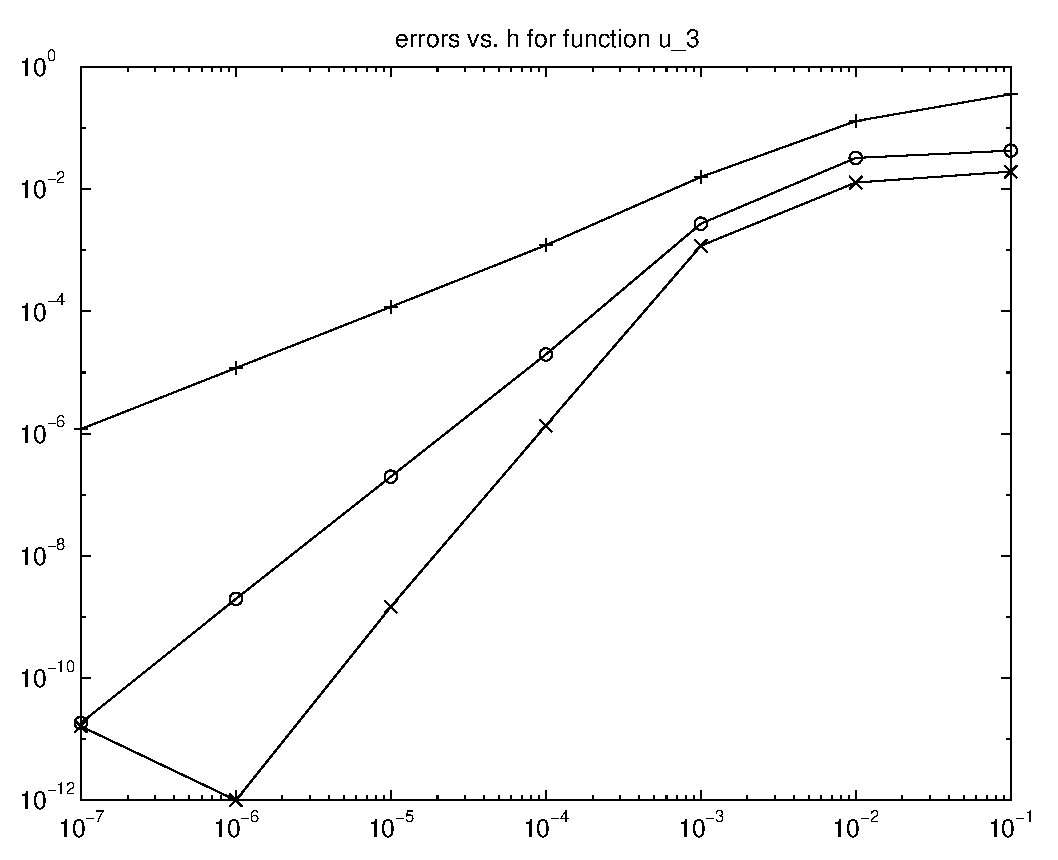
\epsfig{file=err3.eps,width=3in}\hfil
\caption{Log-log plot of errors vs.\ $h$ for test function $u_3$.
$+=D_+$, $o=D_0$, $\times = D_3$.}
\end{figure}


\newpage
A sample matlab m-file is appended that was used to obtain the results
above.  The function is called with specific functions {\tt u} and {\tt
uprime} to specify the test function and its derivative.
The matlab command
\begin{verbatim}
   >> hw0('u1', 'u1prime')
\end{verbatim}
produces the first set of plots and table. 

\vskip 5pt
\hrule
\vskip 5pt

\small
\begin{verbatim}

function hw0(u,uprime)

x = 1;
nh = 7;
errors = ones(nh,4);
ux = feval(u,x);

disp(' ')
disp('         h         D+ error      D_0 error     D_3 error')
disp(' ')

for i=1:nh
  h = 10^(-i);
  up = feval(u,x+h);
  um = feval(u,x-h);
  umm = feval(u,x-2*h);
  dp = (up - ux)/h;
  d0 = (up - um)/ (2*h);
  d3 = (2*up + 3*ux - 6*um + umm) / (6*h);
  dtrue = feval(uprime,x);
  errp = dp-dtrue;
  err0 = d0-dtrue;
  err3 = d3-dtrue;
  errors(i,:) = [h,errp,err0,err3];
  disp(sprintf('  %12.4e  %12.4e  %12.4e  %12.4e',h,errp,err0,err3))
  end

% plot errors:
loglog(errors(:,1),abs(errors(:,2)))
hold on
loglog(errors(:,1),abs(errors(:,2)),'+')
loglog(errors(:,1),abs(errors(:,3)))
loglog(errors(:,1),abs(errors(:,3)),'o')
loglog(errors(:,1),abs(errors(:,4)))
loglog(errors(:,1),abs(errors(:,4)),'x')
hold off


%------------------------------

function u=u1(x)
u = sin(10*x);

%------------------------------

function up=u1prime(x)
up = 10*cos(10*x);

\end{verbatim}


\end{document}
